\documentclass{svproc}

%\documentclass[a4paper, 10pt, conference]{ieeeconf}      % Use this line for a4 paper

\IEEEoverridecommandlockouts                              % This command is only needed if
                                                          % you want to use the \thanks command

\overrideIEEEmargins                                      % Needed to meet printer requirements.

%In case you encounter the following error:
%Error 1010 The PDF file may be corrupt (unable to open PDF file) OR
%Error 1000 An error occurred while parsing a contents stream. Unable to analyze the PDF file.
%This is a known problem with pdfLaTeX conversion filter. The file cannot be opened with acrobat reader
%Please use one of the alternatives below to circumvent this error by uncommenting one or the other
%\pdfobjcompresslevel=0
%\pdfminorversion=4

% See the \addtolength command later in the file to balance the column lengths
% on the last page of the document

% The following packages can be found on http:\\www.ctan.org
\usepackage{graphics} % for pdf, bitmapped graphics files
\usepackage{epsfig} % for postscript graphics files
\usepackage{mathptmx} % assumes new font selection scheme installed
\usepackage{times} % assumes new font selection scheme installed
\usepackage{amsmath} % assumes amsmath package installed
\usepackage{amssymb}  % assumes amsmath package installed
\usepackage{caption}
\usepackage{subcaption}
\usepackage{array}
\usepackage{siunitx}
\usepackage{tabularx}
\usepackage[T1]{fontenc}
\usepackage{makecell}

\title{\LARGE \bf
Laser Tracker Placement Optimization for highly flexible manufacturing systems
}



\author{Jan Baumgärtner$^{1}$,  Alexander Puchta$^{1}$ and Jürgen Fleischer$^{1}$% <-this % stops a space
\thanks{*The authors would like to thank the Ministry of Science, Research and Arts of the Federal State of Baden-Württemberg for the financial support of the project within the InnovationsCampus Future Mobility.
}% <-this % stops a space
\thanks{$^{1}$Jan Baumgärtner, Alexander Puchta, and Jürgen Fleischer are with the wbk Institute of Production Science,
        Karlsruhe Institute of Technology, 76131 Karlsruhe, Germany
        {\tt\small jan.baumgaertner@kit.edu}}%
}



\begin{document}



\maketitle
\thispagestyle{empty}
\pagestyle{empty}


\section{Formulation of the optimization problem}
To solve the joint optimization problem of marker and laser tracker pose we first need to define the objective function.
Our goal is ofcourse to maximize the visibility of the marker to the laser tracker.
Similar to approaches such as \cite{ieee_sensors} we divide the visibility into two components.
Line of sight visibility and field of view visibility.
Both  are depicted in figure \ref{fig:visibility}.
\begin{figure}
        \centering
        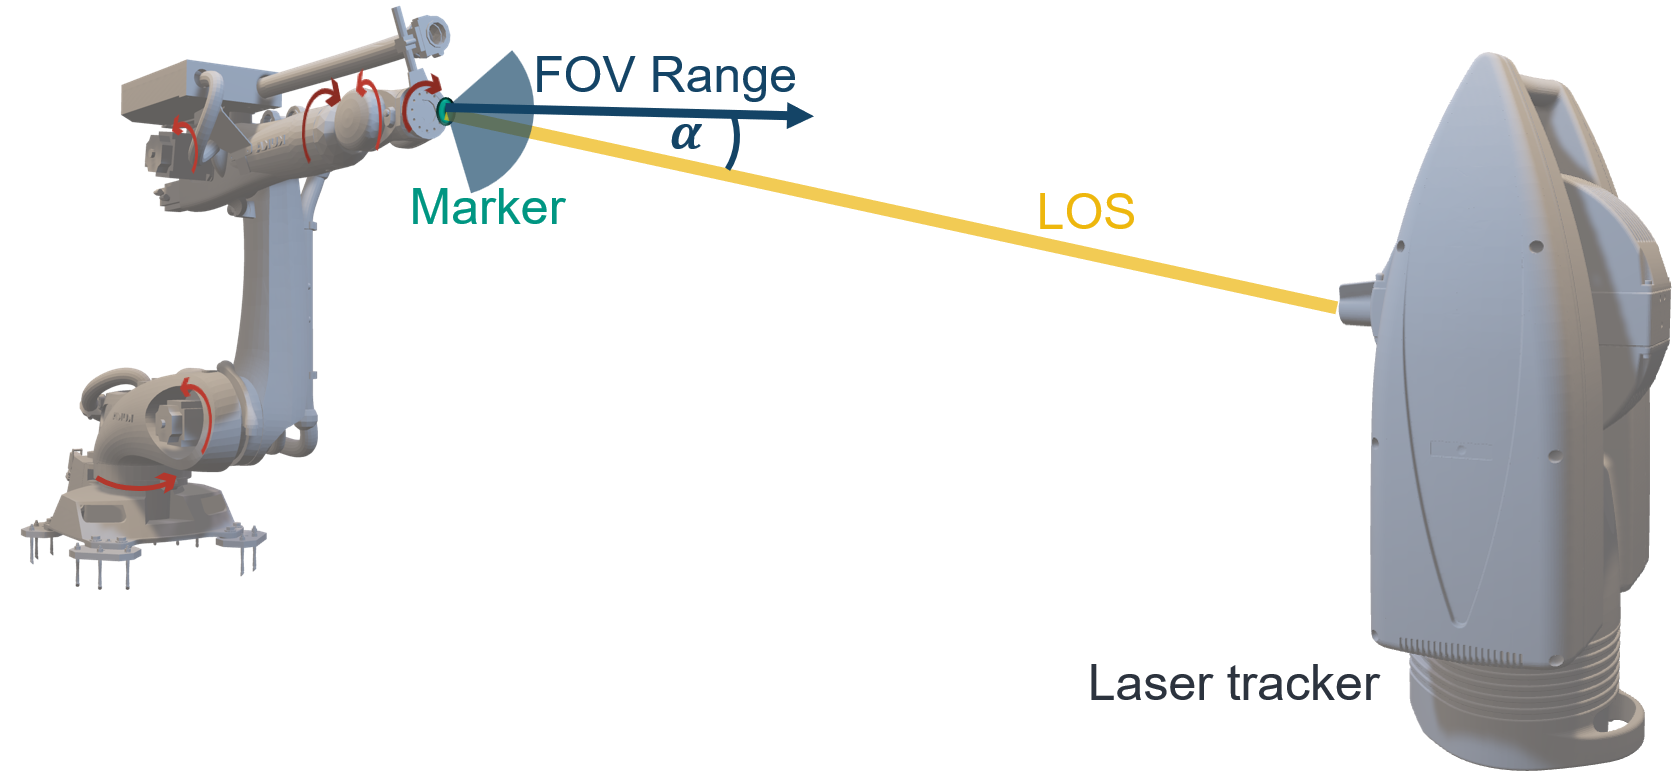
\includegraphics[width=0.8\textwidth]{figures/visibility.png}
        \caption{Field of view (VOW) angle range and line of sight (LOS) components of marker visibility}
        \label{fig:visibility}
\end{figure}
Mathematically we can define line of sight visibility (los visibility) as the following binary function:
\begin{equation}
    f(p_m,p_l) = \begin{cases}
    1 & \text{if } \text{marker is in line of sight of the laser tracker} \\
    0 & \text{otherwise}
    \end{cases}
\end{equation}
where $p_m$ is the position of the marker, $p_l$ is the position of the laser tracker.
Note that $p_m$ is typically dependent on time as it is attached to a moving manufacuting system such as a robot.
The field of view objective can similarly be defined as a binary function:
\begin{equation}
    g(p_m,p_l) = \begin{cases}
    1 & \text{if } \text{marker is in the field of view of the laser tracker} \\
    0 & \text{otherwise}
    \end{cases}
\end{equation}
However in practice it might make sense to not be close to the boundary of the field of view.
Instead one can define a continuous function that is 1 in the center of the field of view and 0 at the boundary.
The simplest way to encode this using the angle $\alpha$ between the normal of the marker and the line of sight of the laser tracker.
\begin{equation}
    g(p_m,p_l) = \cos(\alpha)
\end{equation}
The final objective function is then a weighted sum of the two components:
\begin{equation}
    h(p_m,p_l) = \lambda f(p_m,p_l) + (1-\lambda) g(p_m,p_l)
    \label{eq:objective}
\end{equation}
where $\lambda$ is a weighting factor between 0 and 1 that can be adjusted to prioritize one component over the other.
After defining the objective function we can now define the design variables and constraints.
The design variables are the pose of the laser tracker $p_l$ and the pose of the marker $p_m$.
However the pose of these objects is not arbitrary.
For the purposes of this paper we assume that the marker is attached to the flange of the manufacturing system.
This means that we only define a Transformation matrix $T_{m}$ that describes the pose of the marker relative to the flange.
The final pose of the marker $p_m$ is then given by the flange transformation $T_{f}(q)$ where $q$ is the joint configuration of the robot as well as the transformation $T_{m}$:
\begin{equation}
    p_m = T_{f}(q)T_{m}
\end{equation}
While the matrix $T_m$ is a 4x4 matrix, we can parameterize it using the position of the marker $p_{p_m}$ and the orientation of the marker $p_{o_m}$.
This results in a 6 dimensional design space for the marker pose.
This space is further constraint to avoid any unrealistic marker positions (such as 10 meters above the robot).
Ideally the marer should be attached close to the surface of the manufacutring system to avoid any unneccessarily large constructions that might collide with the environment or cause vibrations.
This can be encoded using a cylindrical constraint on the position of the marker:
\begin{equation}
        \begin{split}
    \sqrt{p_{p_m,x}^2 + p_{p_m,y}^2} &\leq r \\
        0 \leq p_{p_m,z} &\leq h
        \end{split}
\end{equation}
where $r$ is the radius of the cylinder and $h$ is the height of the cylinder.
The marker of course also cant be within the mesh of the manufacturing system, but since this would result in a line of sight visibility of 0 we do not need to encode this constraint explicitly.


The pose of the laser tracker is in reality also defined by a transformation matrix $T_{l}$.
However since the laser tracker has a spherical measurment volume we only need to define the position of the laser tracker $p_{p_l}$, which is a three dimensional vector.
The laser tracker is also mounted on a stand, in principle this can vary in height but only in a limited range.
This can be encoded using a simple constraint:
\begin{equation}
    h_{min} \leq p_{p_l,z} \leq h_{max}
\end{equation}
where $h_{min}$ and $h_{max}$ are the minimum and maximum height of the laser tracker stand.
The laser tracker also has a limited range of measurement.
Here we can define a constraint that the distance between the laser tracker and the marker is within the range of the laser tracker:
\begin{equation}
    d_{min} \leq ||p_{p_m} - p_{p_l}|| \leq d_{max}
\end{equation}
where $d_{min}$ and $d_{max}$ are the minimum and maximum range of the laser tracker.
The final design space is then 9 dimensional, 6 for the marker pose and 3 for the laser tracker pose.

\section{Optimization algorithm}
There are a large number of possible optimization algorithms that can be used to solve this problem.
Following the no free lunch theorem we want to pick the algorithm that makes the most use of the underlying structure of the problem. %TODO citation needed
In this case the problem is a continuous optimization problem with a relatively low number of design variables.
On the other hand it is a gradient free optimization problem due to the line of sight visibility function.
These two properties make the problem well suited for the particle swarm optimization (pso) algorithm.
Particle swarm optimization (PSO) is a computational method for finding the optimal solution to a problem
 It is inspired by the behaviour of swarms in nature, such as flocks of birds or schools of fish, which exhibit emergent behaviour that is intelligent and efficient.
 In PSO, a group of particles (also called agents or individu-als) move through a search space, according to the fol-lowing update rules:
\begin{equation}
        \begin{split}
        x_{i,j} &= x_{i,j} + v_{i,j} \\
    v_{i,j} &= wv_{i,j} + c_1r_1(p_{i,j}-x_{i,j}) + c_2r_2(p_{g,j}-x_{i,j})
        \end{split}
\end{equation}
where $x_{i,j}$ is the position of particle $i$ in dimension $j$, $v_{i,j}$ is the velocity of particle $i$ in dimension $j$, $w$ is the inertia weight,
 $c_1$ and $c_2$ are the cognitive and social coefficients, $r_1$ and $r_2$ are random numbers between 0 and 1, $p_{i,j}$ is the best position of particle $i$ in dimension $j$ and $p_{g,j}$
is the best position of the swarm in dimension $j$.
In our case the particles are a 9 dimensional vector based on the position of the laser tracker and the pose of the marker.
The best particle is the one that maximizes the objective function defined in equation \ref{eq:objective}.
The hyperparameters we need to tune are collected in table \ref{tab:hyperparameters}.
Note that the pso algorithm has no direct way to encode the constraints we defined earlier.
Instead we can use a penalty function that penalizes any particles that violate the constraints.
This is a common approach in optimization and is also used in the implementation of the pso algorithm in the scipy library. %TODO citation needed
The penalty function can be defined as:
\begin{equation}
    p(x) =  \begin{cases}
        0 & \text{if } x \text{ satisfies all constraints} \\
        -\rho & \text{otherwise}
    \end{cases}
\end{equation}
where $\rho$ is a large penalty factor.


\begin{table}  %TODO anpassen
        \centering
        \begin{tabular}{c|c}
                Hyperparameter & Value \\
                \hline
                Number of particles & 100 \\
                Number of iterations & 1000 \\
                Inertia weight & 0.9 \\
                Cognitive coefficient & 2.0 \\
                Social coefficient & 2.0 \\
        \end{tabular}
        \caption{Hyperparameters of the PSO algorithm}
        \label{tab:hyperparameters}
\end{table}

\section{Simulation Environment}
Evaluating the objective function requires a simulation of the manufacturing system.
The tricky part here is that since the manufacturing is actively manufacturing parts we not only need to simulate the behavior of the system itself but the changing shape of any parts that are being manufactured.
For this purpose we are using the pybullet-industrial package \cite{pybullet_industrial}.
This extension of the pybullet physics engine allows us to simulate not only the robot but also the manufacturing process.
For the purposes of this paper the markers are implemented as a pybullet industrial endeffector obect that is attached to the robot.
A image of the simulation environment is shown in figure \ref{fig:simulation}.
\begin{figure}
        \centering
        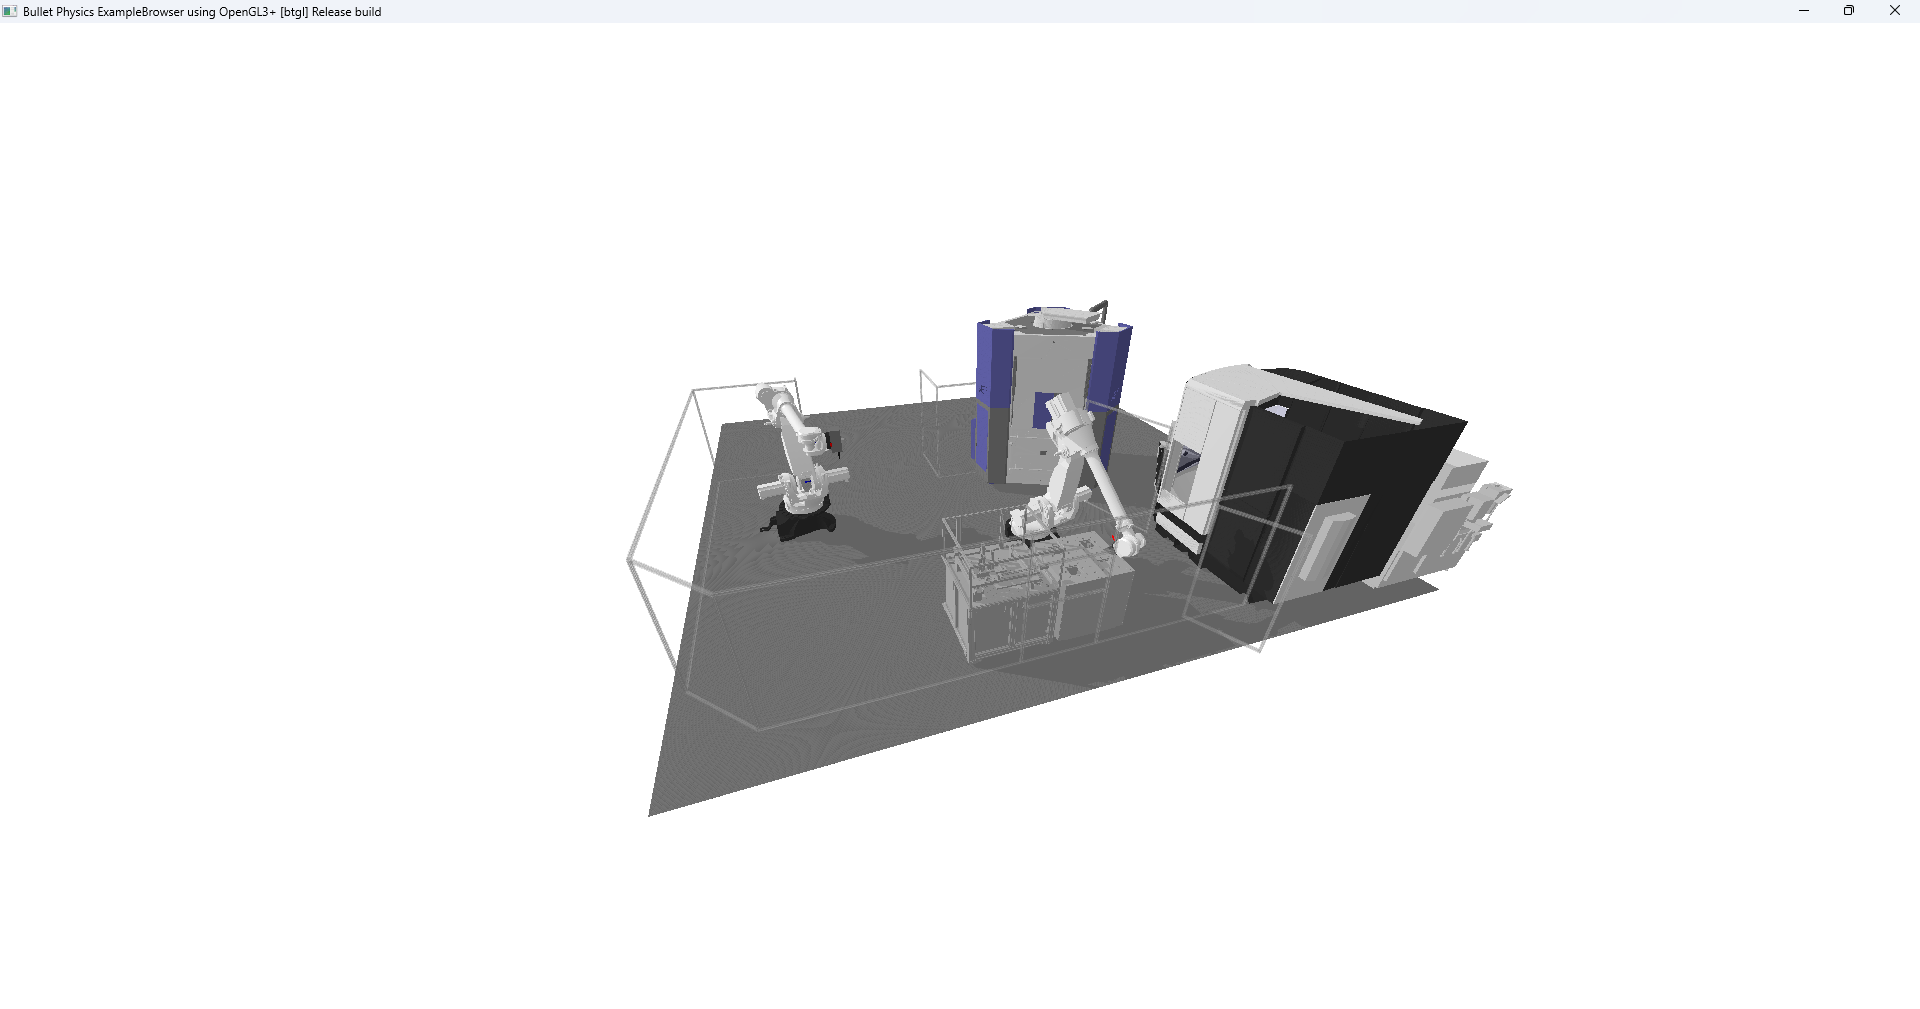
\includegraphics[width=\textwidth]{figures/simulation.png}
        \caption{Simulation environment used for the optimization}
        \label{fig:simulation}
\end{figure}

\section{Experiment Setup}
To test the performance of our optimiser, we need to define a set of test cases.
These consist of different trajectories of the two robots shown in figure \ref{fig:simulation}.
Both robots are Comau NJ290 industrial robots with a reach of 2.9 metres.
The right robot is used to service the CNC machine and the additive manufacturing system, while the left robot is used to perform a high-precision manufacturing task.
To properly control this task, the left robot needs to be tracked by the laser tracker.
We test whether our algorithm is able to find a placement of the laser tracking system and markers that can track the robot over its entire trajectory.
We compare this to the performance of the original population of marker and laser tracker placements used to start the optimisation.





\end{document}

